\documentclass[english, 12pt]{beamer}
% Add handout to documentclass options if wanted

\usepackage[utf8]{inputenc}
\usepackage[T1]{fontenc}
\usepackage{babel,textcomp}


\usepackage{graphicx}
\usepackage{amsmath}
\usepackage{amssymb}
\usepackage{amsbsy}
\usepackage{amsfonts}
\usepackage{color}
\usepackage{xcolor}
\usepackage{epstopdf}
\usepackage{fancyvrb}
\usepackage{parskip}
\usepackage{url}
\usepackage{listings}

\DeclareMathAlphabet{\mathbfit}{OML}{cmm}{b}{it}

\definecolor{javared}{rgb}{0.6,0,0} % for strings
\definecolor{javagreen}{rgb}{0.25,0.5,0.35} % comments
\definecolor{javapurple}{rgb}{0.5,0,0.35} % keywords
\definecolor{javadocblue}{rgb}{0.25,0.35,0.75} % javadoc

\lstset{language=python,
basicstyle=\ttfamily\scriptsize,
keywordstyle=\color{javapurple},%\bfseries,
stringstyle=\color{javared},
commentstyle=\color{javagreen},
morecomment=[s][\color{javadocblue}]{/**}{*/},
% numbers=left,
% numberstyle=\tiny\color{black},
stepnumber=2,
numbersep=10pt,
tabsize=4,
showspaces=false,
captionpos=b,
showstringspaces=false,
frame= single,
breaklines=true}


\setlength{\arrayrulewidth}{1.6pt}
\renewcommand{\arraystretch}{1.2}
\newlength{\Tcalc}


\setbeamertemplate{frametitle}
{\begin{centering}\smallskip
\insertframetitle\par
\smallskip\end{centering}}
\setbeamertemplate{itemize item}{$\bullet$}
\setbeamertemplate{navigation symbols}{}
\setbeamertemplate{footline}[text line]{%
\hfill\strut{%
\scriptsize\sf\color{black!60}%
\quad\insertframenumber
   }%
    \hfill
}

% Define some colors:
\definecolor{DarkFern}{HTML}{407428}
\definecolor{DarkCharcoal}{HTML}{4D4944}
\colorlet{Fern}{DarkFern!85!white}
\colorlet{Charcoal}{DarkCharcoal!85!white}
\colorlet{LightCharcoal}{Charcoal!50!white}
\colorlet{AlertColor}{orange!70!black}
\colorlet{DarkRed}{red!70!black}
\colorlet{LightBlue}{blue!70!white}
\colorlet{DarkBlue}{blue!70!black}
\colorlet{DarkGreen}{green!70!black}

% Use the colors:
\setbeamercolor{title}{fg=Fern}
\setbeamercolor{frametitle}{fg=Fern}
\setbeamercolor{normal text}{fg=Charcoal}
\setbeamercolor{block title}{fg=black,bg=Fern!25!white}
\setbeamercolor{block body}{fg=black,bg=Fern!25!white}
\setbeamercolor{alerted text}{fg=AlertColor}
\setbeamercolor{itemize item}{fg=Charcoal}

\newcommand{\frn}[1]{\textcolor{Fern}{#1}}
\newcommand{\alrt}{\color{AlertColor}}
\newcommand{\bt}[1]{\textbf{#1}}
\newcommand{\kommando}[1]{\textcolor{AlertColor}{\texttt{\textbackslash #1}}}
\newcommand{\ds}{\displaystyle}

\renewcommand{\d}{\textrm{d}}

\title{Programmeringsprosjekt Sandvika \\ {\small En introduksjon til numeriske beregninger}}
\author{Jonas van den Brink \\ \texttt{j.v.brink@fys.uio.no}}
\institute{\alrt Simula Research Laboratory \\ Oslo, Norway}

\setbeamertemplate{frametitle}{\vspace{0.5cm} \insertframetitle} 

\begin{document}
\pagestyle{empty}

\begin{frame}
\maketitle 
\end{frame}

\begin{frame}[fragile]
\frametitle{La oss starte med verktøyene vi trenger}

Vi kommer til å programmere i programmeringsspråket {\alrt Python}.

\visible<2-> {
	
For å installere alt vi trenger er det enklest å installere \emph{\alrt Enthought Canopy}. Det er gratis og enkelt.

{\color{DarkFern} \url{https://store.enthought.com/downloads/}}

Pakken er tilgjengelig på Windows, Mac og Linux.
}

\vspace{1cm}

\visible<3-> {
Bruker du Linux har du nok allerede Python installert, og Canopy er ikke nødvendig.	
}
\end{frame}



\begin{frame}[fragile]
\begin{center}
{\Huge \color{DarkFern} Hva er det vi skal gjøre?}

\vspace{1cm}

Hva vi ønsker å finne ut av \\ og hvordan vi skal gjøre det
\end{center}
\end{frame}

\begin{frame}[fragile]
\frametitle{Målet i mekanikk er å finne bevegelsen til et legeme.}

\begin{center}
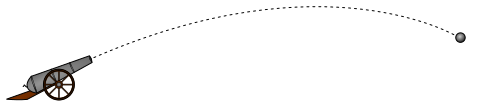
\includegraphics[width=\textwidth]{cannonball}
\end{center}

\vspace{1cm}

Vi ønsker å finne hastigheten og posisjonen, $\alrt \vec{v}(t)$, $\alrt \vec{r}(t)$, som funksjoner av tid.

\end{frame}

\begin{frame}
\frametitle{Eksempel: Vertikalt kast}

Vi kaster en tennisball rett opp i lufta med en starthastighet på 10 m/s fra 1 m over bakken.

\begin{center}

\includegraphics[width=\textwidth]{tennisball}
\end{center}

\textbf{Oppgave:} Finn hastigheten og høyden over bakken som funksjoner av tid: $\alrt y(t)$, $\alrt v(t)$. Se bort ifra luftmotstand.
\end{frame}

\begin{frame}
\frametitle{Løsning: Vertikalt kast}

\vspace{-1cm}

\begin{align*}
\alrt v(t) &\alrt=  v_0 - gt, \\
\alrt y(t) &\alrt=  y_0 + v_0t - \frac{1}{2}gt^2.
\end{align*}

\vspace{-0.5cm}

\begin{center}
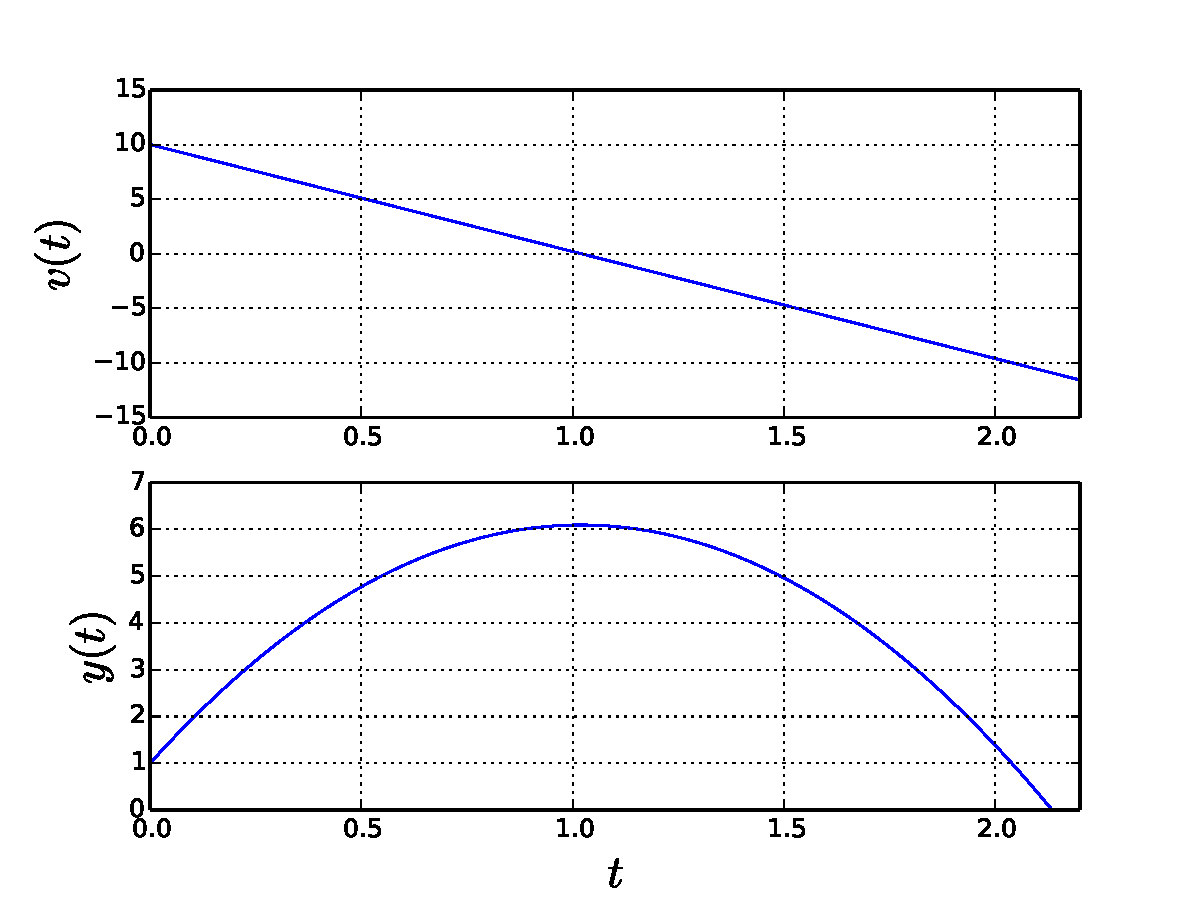
\includegraphics[width=0.75\textwidth]{solvert}
\end{center}
\end{frame}

\begin{frame}
\frametitle{Det vi egentlig har gjort nå er å løse bevegelsesligningene}

$$\alrt \frac{\d x}{\d t} = v(t), \qquad \frac{\d v}{\d t} = a(t).$$

Dette er eksempler på det som kalles $\alrt differensialligninger$. Man lærer mer om dem i R2.

\visible<2-> {
Hvis akselerasjonen er konstant har disse ligningene velkjente løsninger
\begin{align*}
\alrt v(t) &\alrt= v_0 + at,\\
\alrt x(t) &\alrt= x_0 + v_0t + \frac{1}{2}at.	
\end{align*}
}
\end{frame}

\begin{frame}
\frametitle{Hva om akselerasjonen \emph{ikke} er konstant?}

Da må vi løse differensialligningene direkte. Det er ofte vanskelig og i mange tilfeller umulig.

\vspace{1cm}

\visible<2-> {
Man kan bruke numeriske beregninger på datamaskin for å løse differensialligninger.
}

\vspace{1cm}

\visible<3-> {
Dere skal lære å gjøre dette, dere skal programmere et verktøy som kan løse bevegelsesligningene for en \emph{hvilken som helst} akselerasjon.
}
\end{frame}

\begin{frame}
\frametitle{Hvordan finner vi egentlig akselerasjonen?}

\visible<2-> {
	Vi bruker Newtons 2.\ lov, som lar oss finne akselerasjonen fra kreftene som virker på et legeme
	$$\alrt F = ma.$$
}

\visible<3-> {
	Generelt sett kan kreftene på et legeme avhenge av tid, posisjon og fart
	$$\alrt F(x,v,t).$$
}
\end{frame}

\begin{frame}
\frametitle{Hva vi skal gjøre }

Vi kan finne bevegelsen til et legeme ved følgende steg:
\begin{enumerate}
\item Finne kreftene på legemetet ved å analysere fysikken
\item Bruke Newtons 2.\ lov til å finne akselerasjonen
\item Løse bevegelsesligningene (differensialligninger)
\end{enumerate}
\end{frame}

\begin{frame}
\frametitle{Hva vi skal gjøre }



Vi skal regne ut bevegelsen i fallskjermhopp og strikkhopp. Vi bruker da programmering for å løse bevegelsesligningene.

\vspace{0.5cm}

\begin{center}
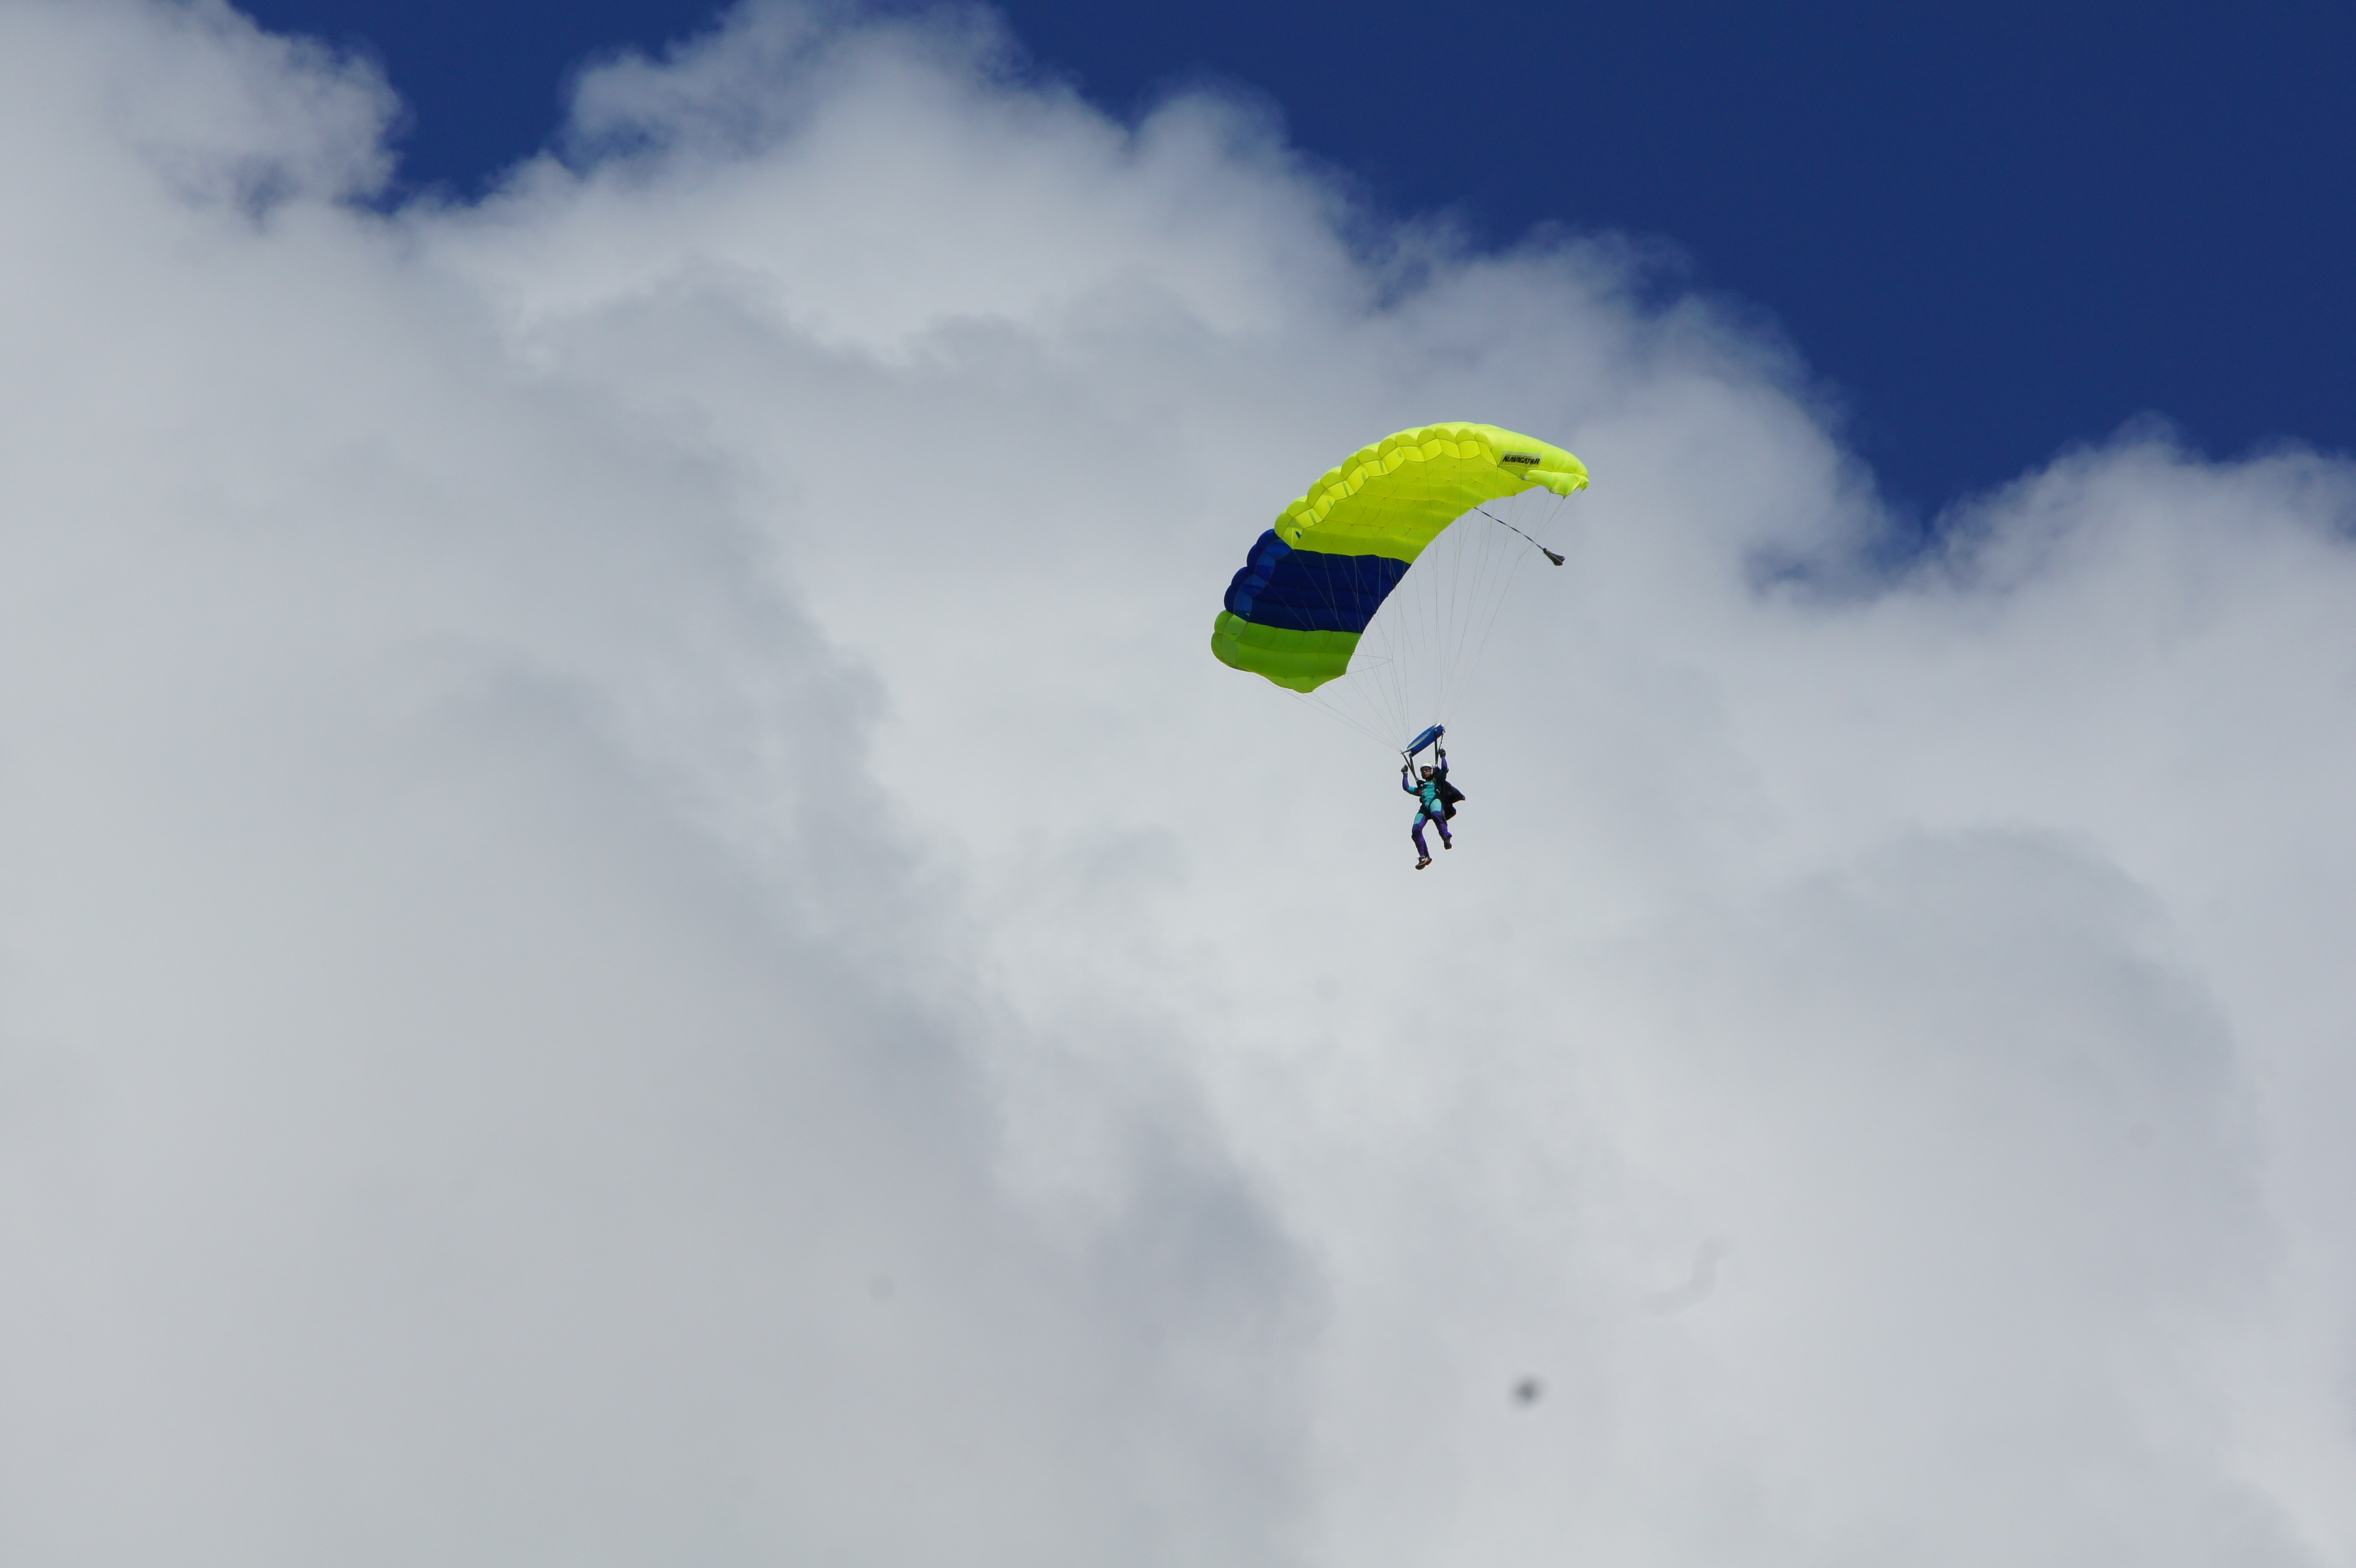
\includegraphics[width=0.75\textwidth]{skydiving}
\end{center}
\end{frame}





% \begin{frame}[fragile]
% \frametitle{We can solve the equations of motion numerically using the Euler method}

% \visible<2-> {	
% From the definition of the derivative
% \begin{align*}
% \alrt \frac{\d v}{\d t} = \lim_{\Delta t \to 0} \frac{v(t+\Delta t) - v(t)}{\Delta t} =  a(t)
% \end{align*}
% }

% \visible<3-> {
% We now remove the limit, making $\Delta t$ a very small constant
% \begin{align*}
% \alrt \frac{v(t+\Delta t) - v(t)}{\Delta t} \approx  a(t)
% \end{align*}
% }

% \visible<4-> {
% Solving for $v(t+\Delta t)$ gives
% \begin{align*}
% \alrt v(t+\Delta t) \approx v(t) + a(t)\cdot \Delta t
% \end{align*}
% }
% \end{frame}

% \begin{frame}[fragile]
% \frametitle{We can solve the equations of motion by stepping forward in time}

% \begin{align*}
% \alrt v(t+\Delta t) = v(t) + a(t)\cdot \Delta t
% \end{align*}
% \visible<2-> {	
% If $a(t)$ and $v(t)$ are known, we can calculate $v(t+\Delta t)$
% }

% \visible<3-> {
% \vspace{-0.2cm}
% \begin{center}
% 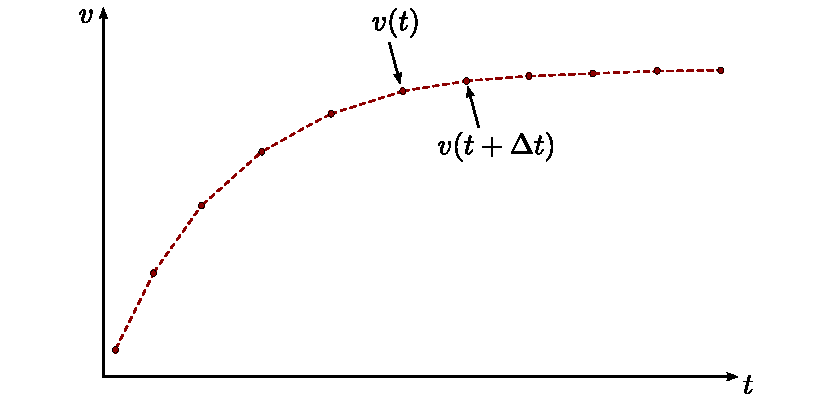
\includegraphics[width=\textwidth]{eulers0.pdf}
% \end{center}
% }
% \end{frame}

% \begin{frame}[fragile]
% \frametitle{Our functions are no longer continuous, they have become discretized}

% \visible<2-> {	
% We only focus on multiples of our time-step
% \begin{align*}
% \alrt t & \alrt \in \{ 0,\ \Delta t,\  2\Delta t, \ 3\Delta t,  \ldots \} \\
% \alrt t_i & \alrt \equiv i\cdot\Delta t
% \end{align*}
% }
% \visible<3-> {	
% Introduce the shorthand
% \begin{align*}
% \alrt v(t_i) &\alrt \equiv v_i \\
% \alrt r(t_i) &\alrt \equiv r_i \\
% \end{align*}
% }

% \visible<4-> {
%  \vspace{-0.4cm}
% \begin{center}
% 
\includegraphics[width=\textwidth]{time_discretization.pdf}
% \end{center}
%  \vspace{0.8cm}
% }
% \end{frame}

% \begin{frame}[fragile]
% \frametitle{We solve the equations of motion iteratively}

% $$\alrt v_{i+1} = v_i + a_i\cdot\Delta t$$
% \visible<2->{	
% $$\alrt r_{i+1} = r_i + v_i\cdot \Delta t$$
% }

% \visible<3->{
% For each time step, we must calculate the acceleration
% $$\alrt a_i = a(r_i, v_i, t_i).$$
% }

% \visible<4->{	
% We repeat these steps, starting at our initial conditions $v_0$ and $r_0$, until we have reached our end-time $t_N$
% $$\alrt i = 0,1,2,3,\ldots, N.$$
% }
% \end{frame}

% \begin{frame}[fragile]
% \frametitle{Algorithm for the Euler method}

% for $i=0,1,2,3,\ldots, N-1$:
% \begin{enumerate}
% 	\item Use the previous results $x_i$ and $v_i$ to compute the acceleration: $\alrt a_i = F(x_i, v_i, t_i)/m$.
% 	\item Compute the new velocity: $\alrt v_{i+1} = v_i + a_i\Delta t$.
% 	\item Compute the new position: $\alrt r_{i+1} = r_i + v_i\Delta t$.
% \end{enumerate}
% \end{frame}


% \begin{frame}[fragile]
% \begin{center}
% {\Huge \color{DarkFern} Implementation}

% \vspace{1cm}

% Moving from physics and math to \\ actual computer code
% \end{center}
% \end{frame}

% \begin{frame}[fragile]

% for $i=0,1,2,3,\ldots, N-1$:
% \begin{enumerate}
% 	\item Use the previous results $x_i$ and $v_i$ to compute the acceleration: $\alrt a_i = F(x_i, v_i, t_i)/m$.
% 	\item Compute the new velocity: $\alrt v_{i+1} = v_i + a_i\Delta t$.
% 	\item Compute the new position: $\alrt r_{i+1} = r_i + v_i\Delta t$.
% \end{enumerate}
% \visible<2-> {
% $$\Downarrow$$

% \lstinputlisting{lsteuler.py}
% }

% \visible<3-> {
% We want the code to look as much as possible like the physics and math we write on paper
% $$\alrt t_i \Rightarrow \texttt{t[i]} \qquad  v_i \Rightarrow \texttt{v[i]} \qquad  r_i  \Rightarrow \texttt{r[i]}$$
% }
% \end{frame}

% \begin{frame}[fragile]
% \frametitle{We also need various bookeeping code}

% Here we define the arrays we will be using
% \lstinputlisting{lstarrays.py}
% \end{frame}

% \begin{frame}[fragile]
% \frametitle{We also need various bookeeping code}

% Here we define physical constants for our system and define the function that describes the forces

% \lstinputlisting{lstforce.py}
% This example show the forces acting on the cannonball as it sails through the air
% $$\alrt F(x,v,t) = F_g + F_d(\vec{v}) = -mg\vec{k} - \frac{1}{2}\rho C_D A |\vec{v}|\vec{v}$$
% \end{frame}

% \begin{frame}[fragile]
% \frametitle{As soon as we have solved the equations of motion, we can plot the result}

% \lstinputlisting{lstplotting.py}
% \end{frame}

% \begin{frame}[fragile]
% \begin{center}
% 	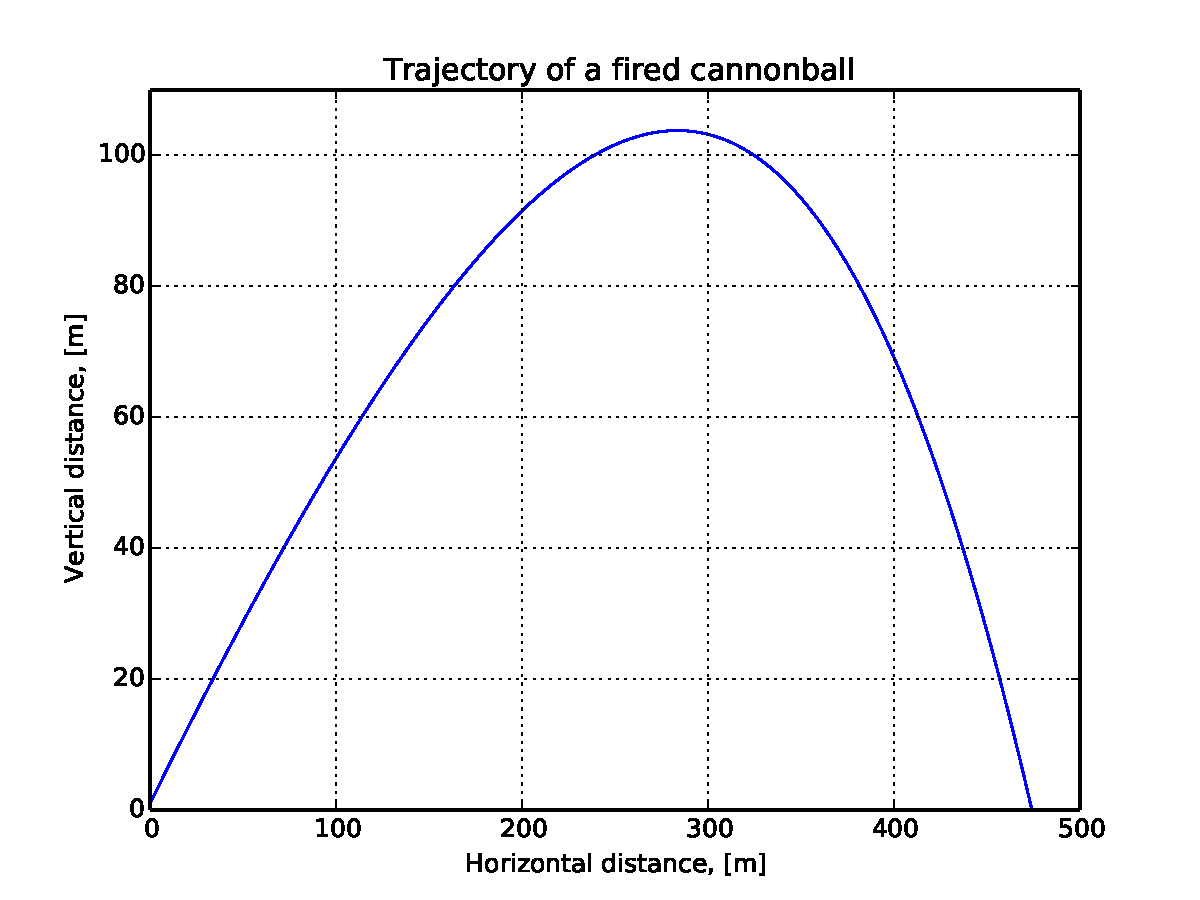
\includegraphics[width=\textwidth]{plot_cannonball1}
% \end{center}
% \end{frame}

% \begin{frame}
% \begin{center}
% {\Huge \color{DarkFern} Numerical Experimentation}

% Altering parameters let's us immediately see the consequences
% \end{center}
% \end{frame}

% \begin{frame}[fragile]
% \begin{center}
% 	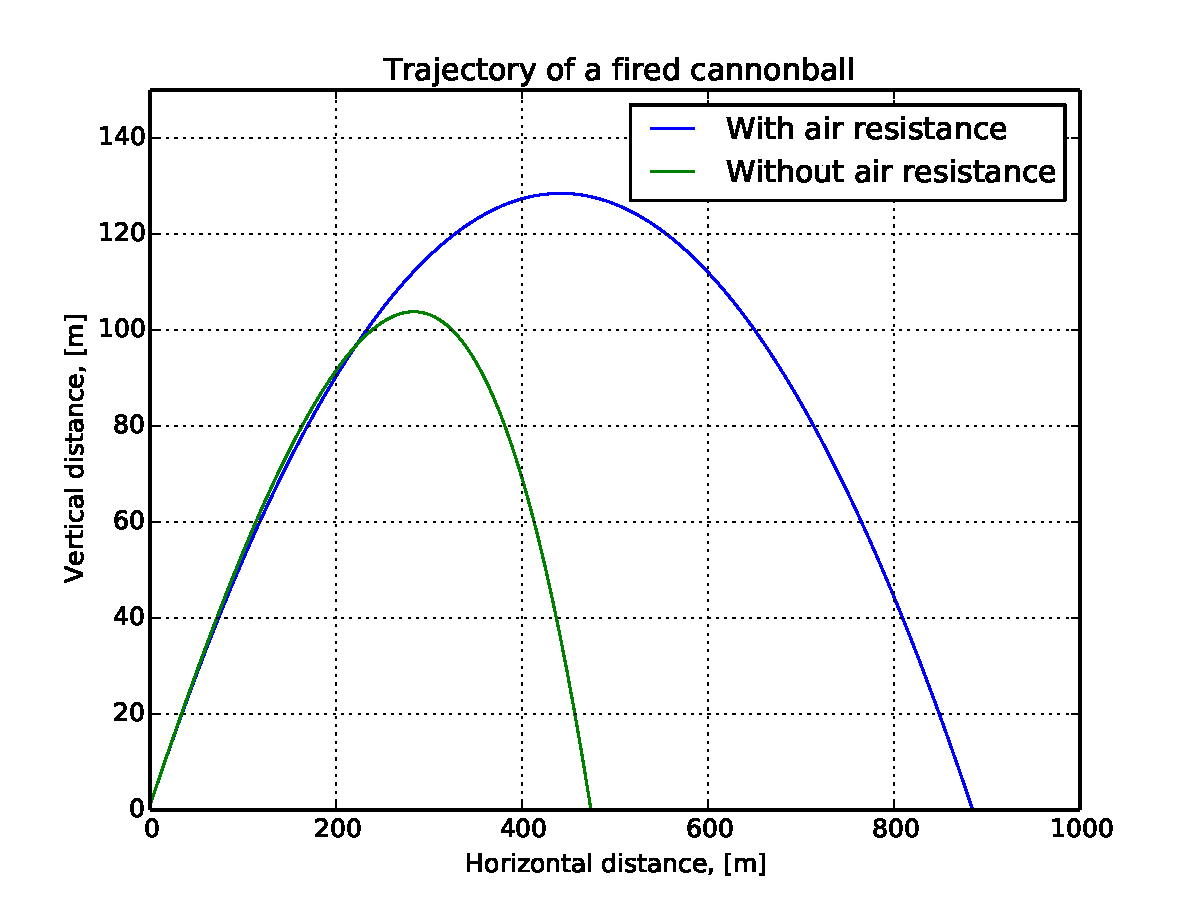
\includegraphics[width=\textwidth]{plot_cannonball2}
% \end{center}
% \end{frame}

% \begin{frame}[fragile]
% \begin{center}
% 	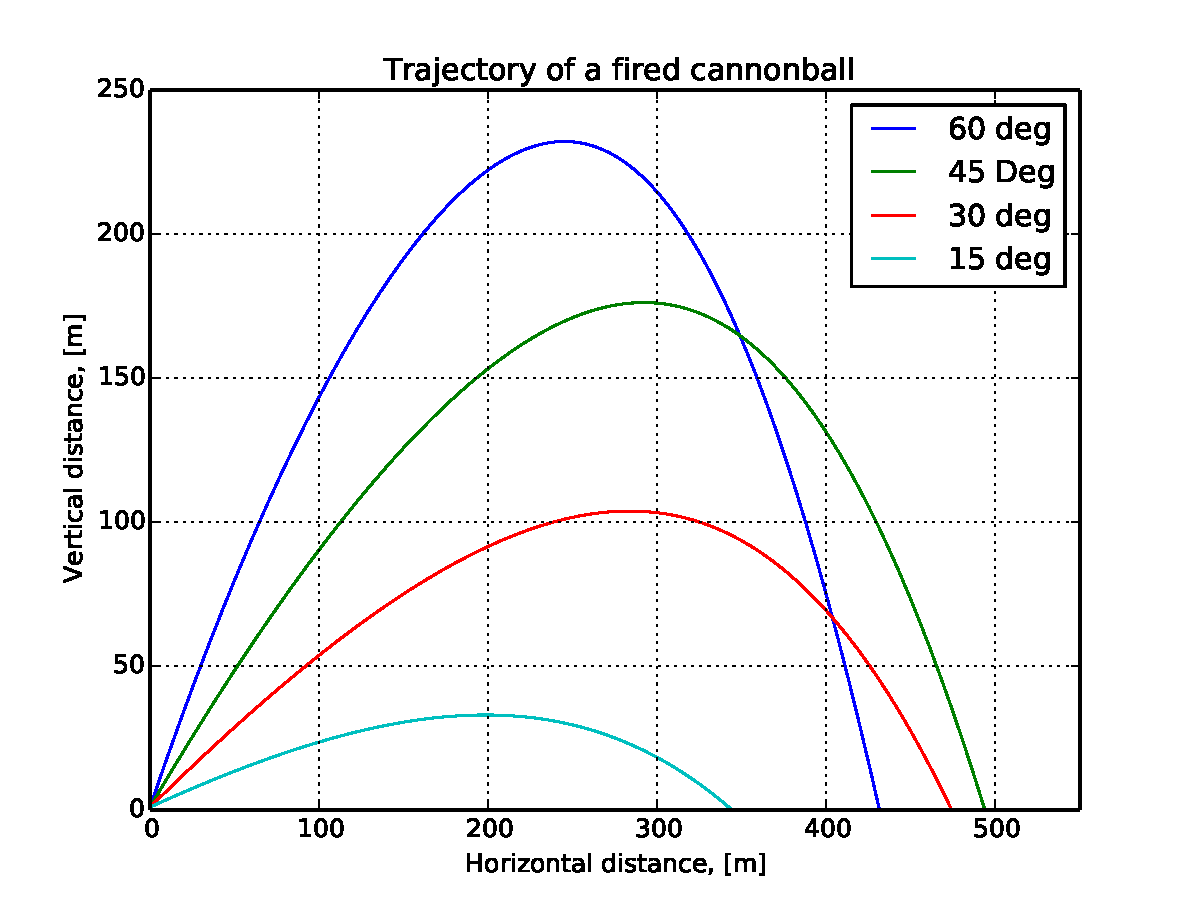
\includegraphics[width=\textwidth]{plot_cannonball3}
% \end{center}
% \end{frame}

% \begin{frame}[fragile]
% \frametitle{Students can use numerical experimentation to build intuition and knowledge}

% \begin{itemize}
% 	\item Numerical results can be compared to known analytical solutions. Are numerical results trustworthy?
% 	\item Can study how results are directly changed by parameter choice. Are the parameters chosen reasonable?
% 	\item Can look at systems with and without certain contributions, such as air drag. \\ What is important, and what can be ignored?
% \end{itemize}
% \end{frame}

% \begin{frame}
% \begin{center}
% {\Huge \color{DarkFern} Examples of possible projects}

% You will have a chance to look at some of these today
% \end{center}
% \end{frame}

% \begin{frame}[fragile]
% \frametitle{Catapults and cannons and sports such as baseball}

% \begin{center}
% 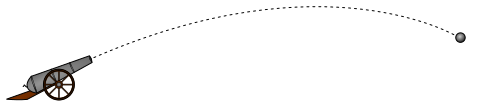
\includegraphics[width=\textwidth]{cannonball}
% \end{center}

% \vspace{0.5cm}

% \begin{itemize}
% 	\item Easy to compare with experimental data, either before or after simulation.
% 	\item Can look into studies of air drag, Reynolds number etc.
% \end{itemize}
% \end{frame}

% \begin{frame}[fragile]
% \frametitle{Skydiving and bungeejumping}

% \begin{center}
% 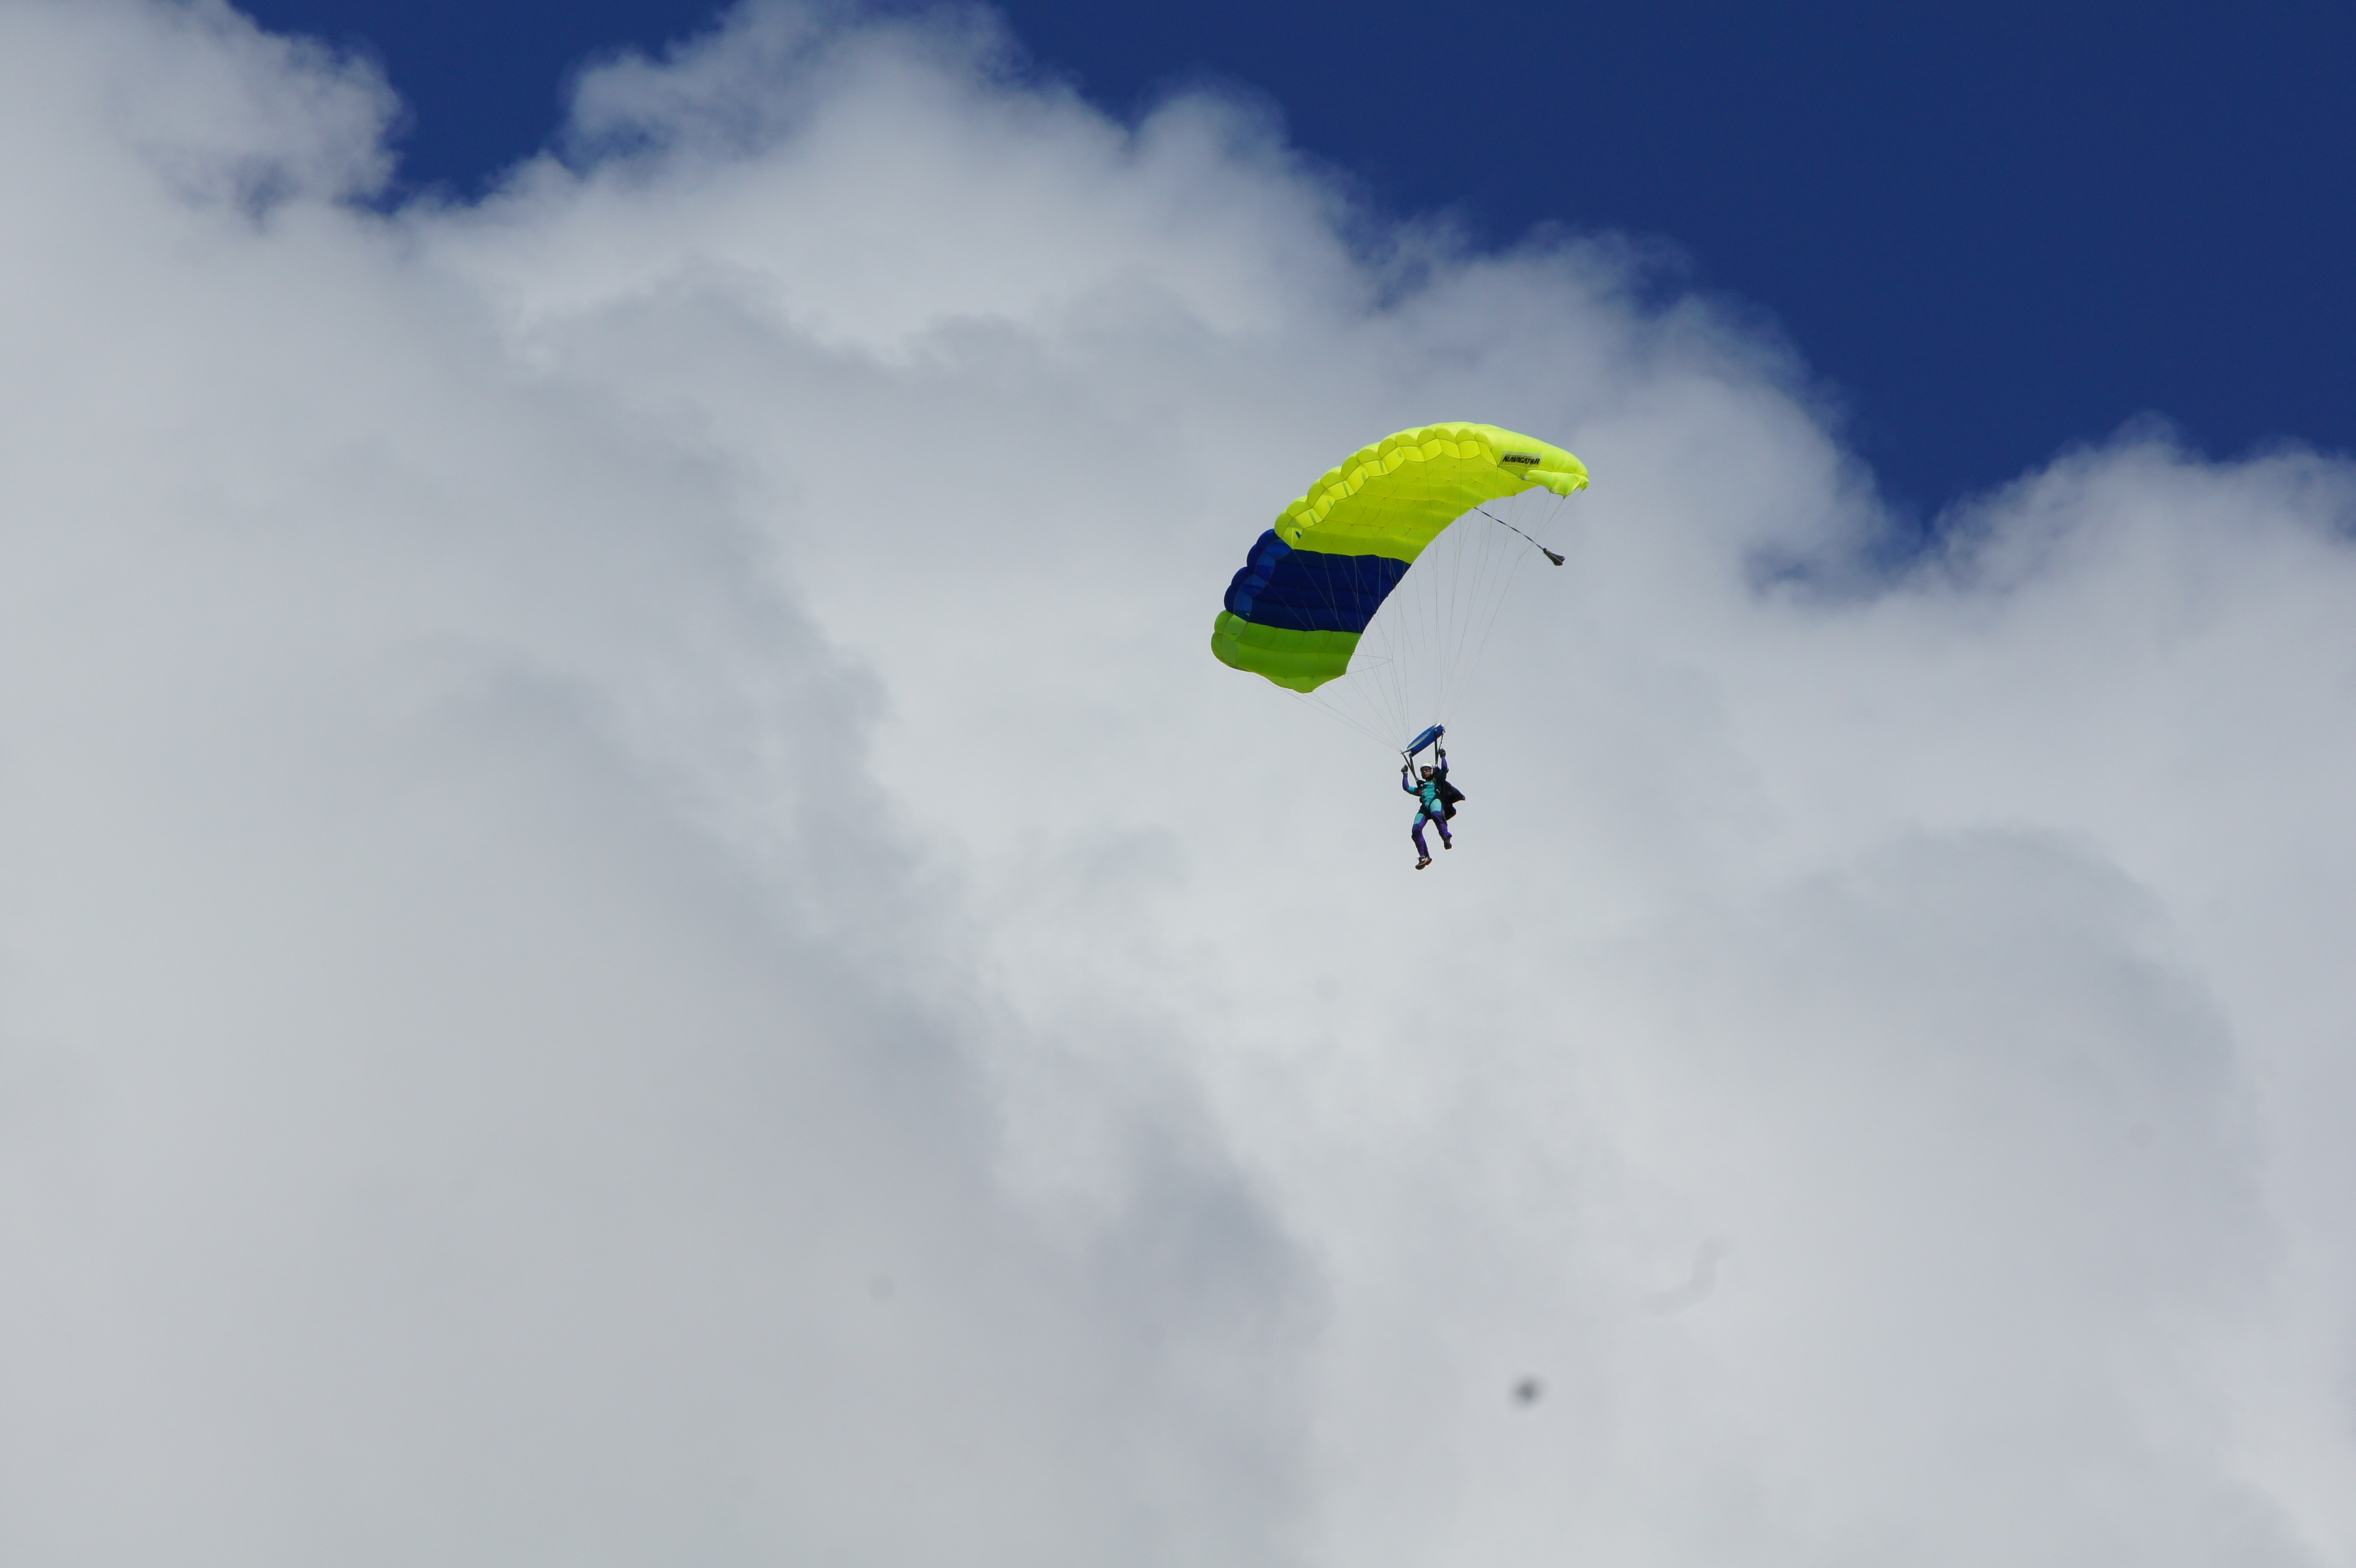
\includegraphics[width=0.6\textwidth]{skydiving}
% \end{center}

% \begin{itemize}
% 	\item Great study on free fall and terminal velocity
% 	\item Can study how parameters such as cross-sectional area and drag coefficient change as the parachute is opened
% 	\item Can plot the $g$-forces affecting the jumper. Which sport is more ``extreme''?
% \end{itemize}
% \end{frame}

% \begin{frame}[fragile]
% \frametitle{Pendulum and angular motion}

% \begin{center}
% 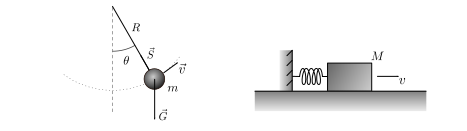
\includegraphics[width=\textwidth]{pendulum}
% \end{center}

% \begin{itemize}
% 	\item Can solve pendulum also for large angles!
% 	\item Energy can be plotted as functions of time
% 	\item Can also simulate double pendulum and chaotic systems
% \end{itemize}
% \end{frame}

% \begin{frame}[fragile]
% \frametitle{Modelling the solar system}

% \begin{center}
% 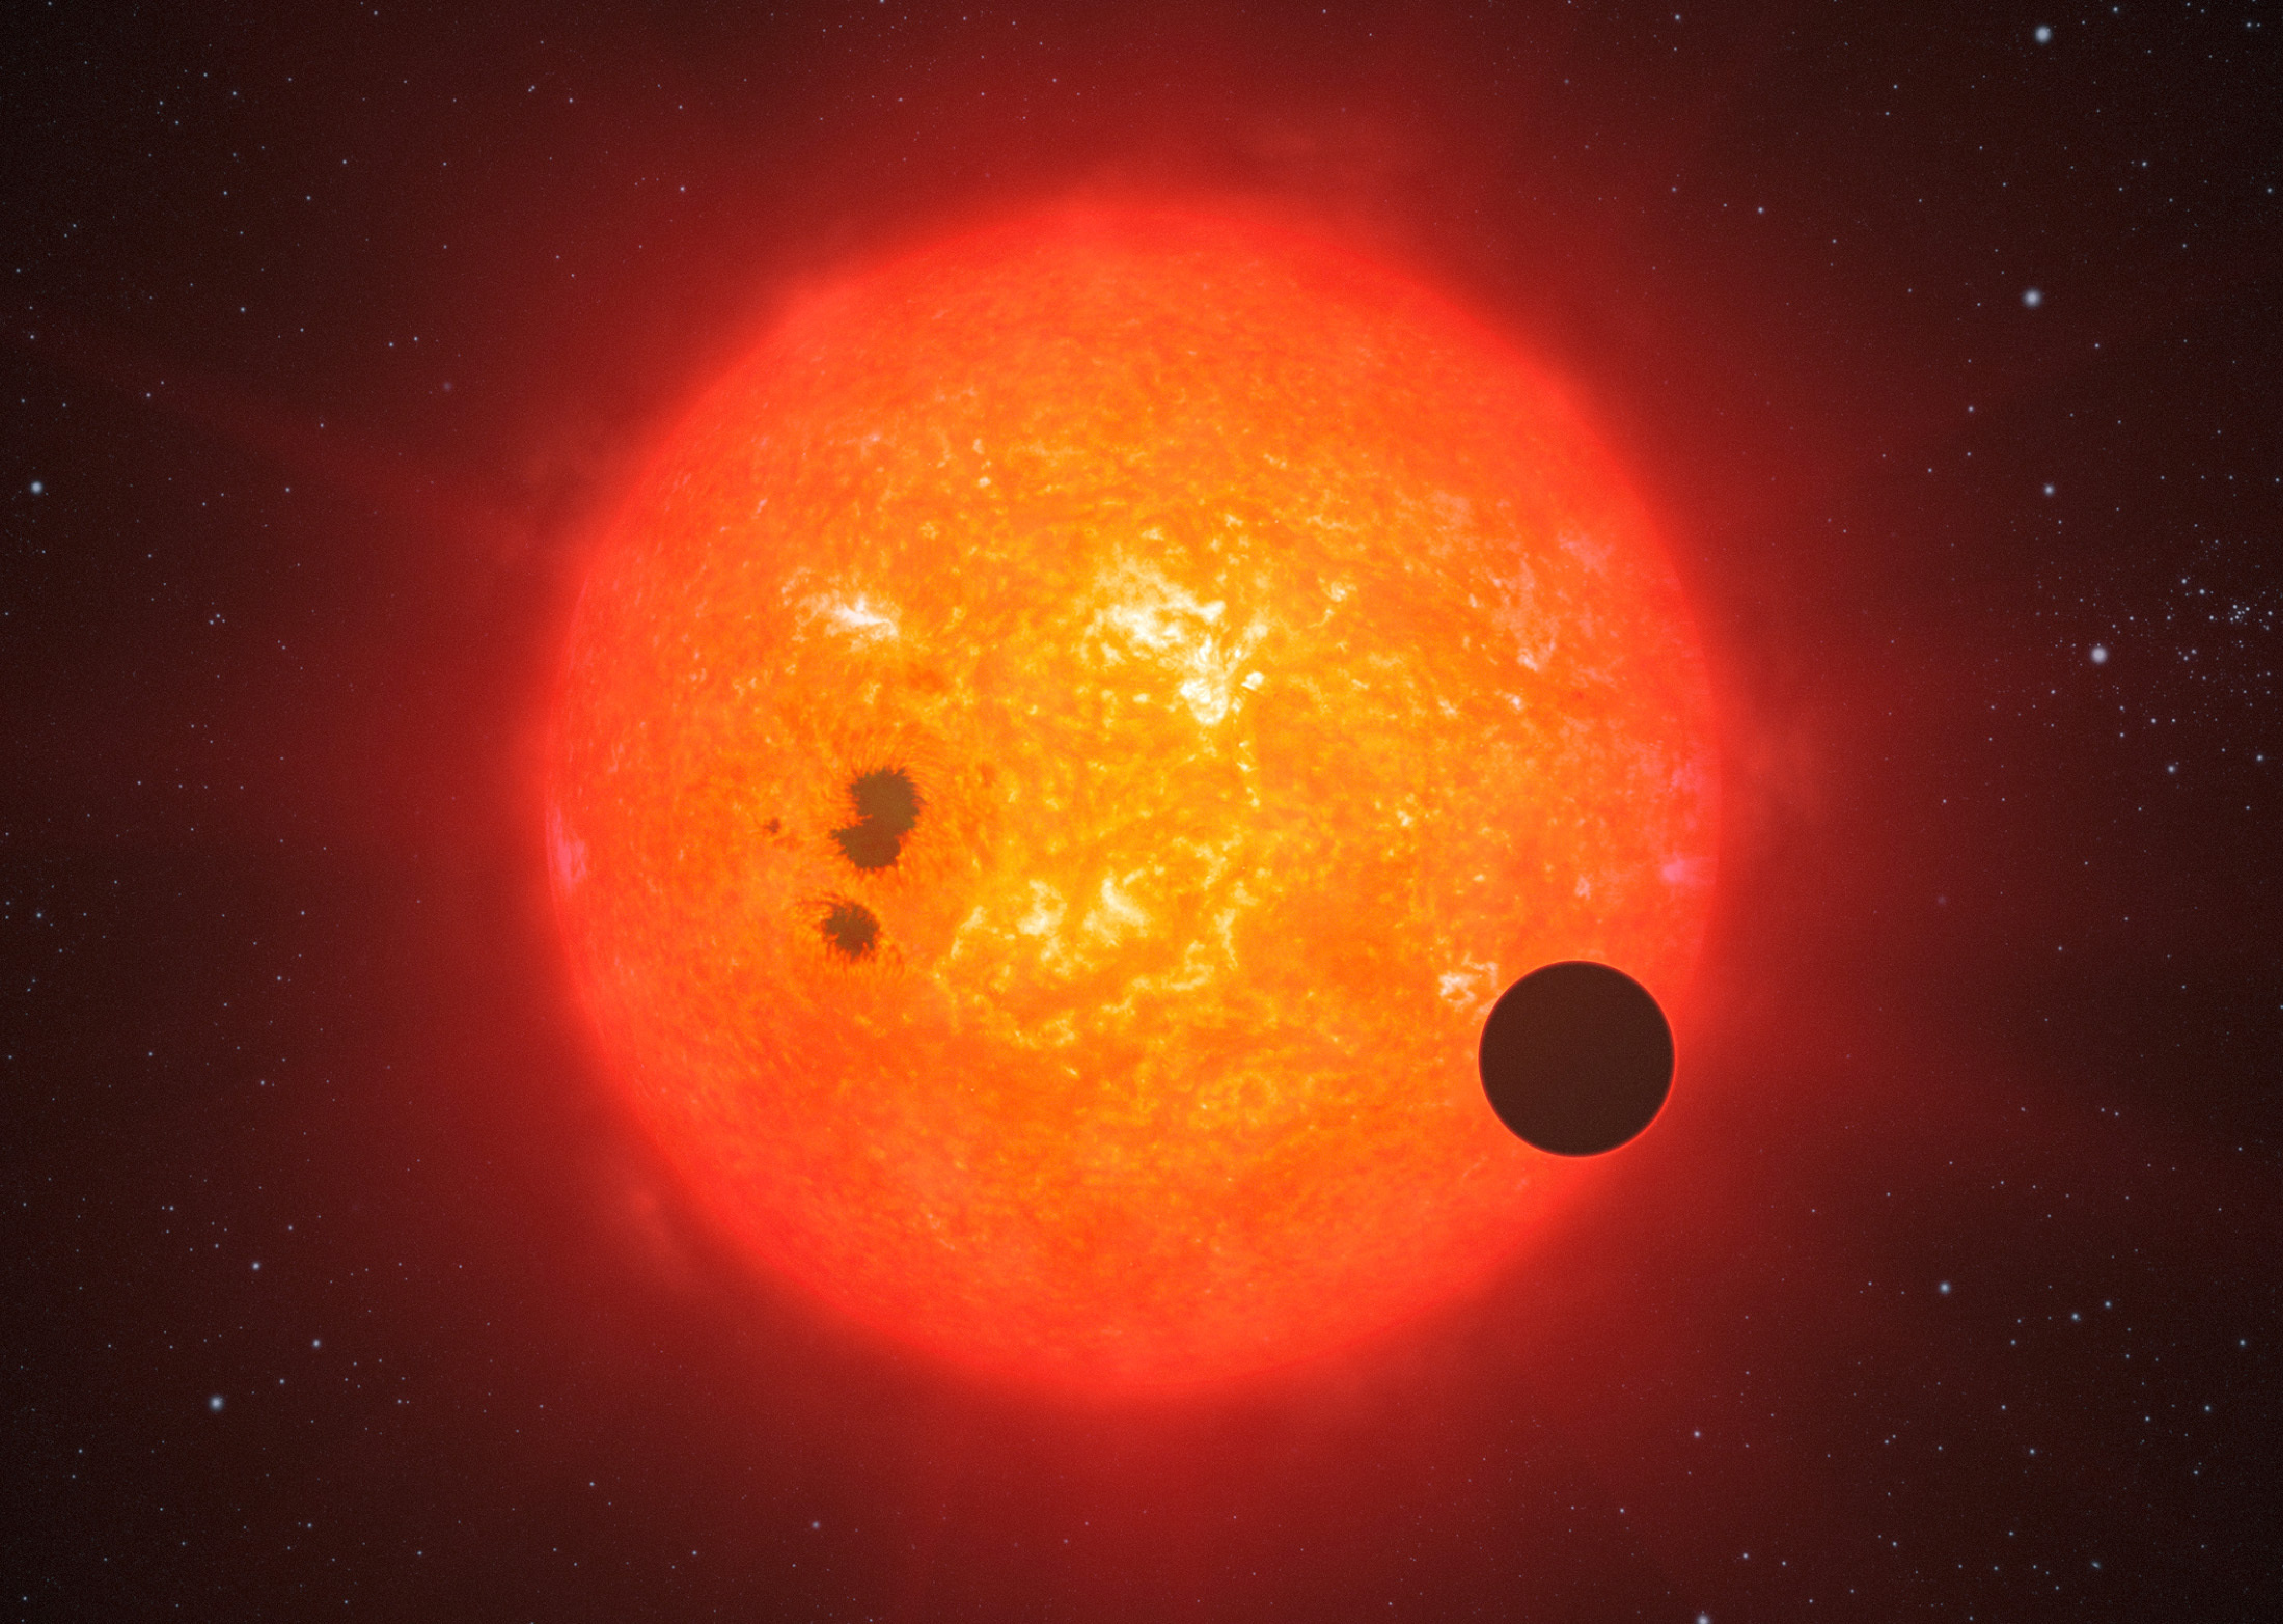
\includegraphics[width=0.4\textwidth]{exopl_GJ1214b_ESO}
% \end{center}

% \begin{itemize}
% 	\item Students can gather real data of planetary orbits from NASA webpages
% 	\item Can combine numerical simulation with better graphics
% \end{itemize}
% \end{frame}


\end{document}